\section{Biološke raziskave razpoznavanja objektov}
Intuicija nam govori, da bomo z razpoznavanjem 3D objektov iz 2D slik zelo težko dosegli človeške zmogljivosti, saj s slikami izgubimo določeno informacijo o naravnih objektih. Kljub temu vemo, da ljudje in opice s pogledom na sliko hitro razpoznajo objekte \cite{rajalingham2018largescale}. Zato so v delu \cite{tarr1998image} raziskovali biološko verodostojnost razpoznavnja 3D objektov iz 2D slik. Primerjali so dva načina modeliranja za rapoznavanje objektov. Slikovni način naj bi bil razmeroma boljši od strukturnega opisa, saj pri slednjem potrebujemo postopek rekonstrukcije \cite{tarr1998image}. Seveda je strukturni opis, s katerim rekonstruiramo 3D objekte bolj robusten od slikovnega načina, saj ta predstavlja izbran objekt samo iz specifičnega pogleda \cite{tarr1998image}. Avtorji \cite{tarr1998image}, vseeno zagovarjajo slikovni način, saj so z raziskavami na opicah pokazali, da v možganih poleg od pogleda neodvisnih nevronov obstajajo tudi taki, ki so aktivni za specifične poglede izbranega objekta. Za razpoznavanje 3D objektov iz 2D slik bi zato za najboljše rezultate morali poleg slikovnih značilk uporabiti strukturno informacijo objekta \cite{tarr1998image}.  

Dodatno potrditev, da so algoritmi razpoznavanja objektov iz 2D slik biološko pomenljivi, so raziskovalci pokazali v delu \cite{leeds2013comparing}. Raziskovali so, kako dobro različni modeli razpoznavanja posnemajo vidno pot v možganih. Pri tem so se osredotočali na starejše modele, ki temeljijo na SIFT značilkah in Gaborjevih filtrih. 

\begin{figure}[!htbp]
	\centering
	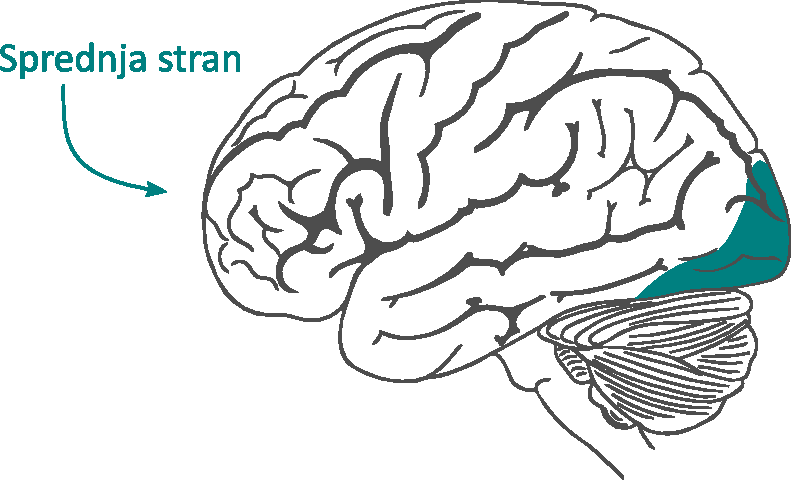
\includegraphics[width=0.7\columnwidth]{leeds_1}
	\caption{Avtor možganov je \cite{brain}.}
\end{figure}


V eksperimentih so uporabili 60 slik objektov na sivem ozadju. Sodelovalo je 5 oseb (moški spol: 4, ženski spol: 1, starost: 20--24 let). Vsako sliko so prikazali za \SI{2}{\s}. Sledila je sivinska slika z naključnim trajanjem med \SI{500}{\ms} in \SI{3000}{\ms}. Na koncu so prikazali še sredinski križec. Pasivno opazovanje slik so merili z MRI napravo. fMRI slike merjencev so povezali z računalniškimi modeli preko reprezentativne disimilarne matrike, ki vsebuje razdalje med objekti. Ker z razdaljo merimo podobnost dveh objektov, disimilarna matrika predstavlja razvrščanje objektov v razrede. 


\citea{leeds2013comparing} je ugotovil, da SIFT daje najboljše rezultate, čeprav so korelacije med modelom in korteksom dokaj nizke (pod \num{0.3}). 

\begin{figure}[!htbp]
	\centering
	\includegraphics[width=0.7\columnwidth]{it_cortex}
	\caption{Avtor možganov je \cite{brain}.}
\end{figure}

V novejših nevroznastvenih raziskavah so raziskovalci ugotovili, da se kategorična informacija za razpoznavanje pojavlja v inferiorni senčni skorji (tudi inferiorni temporalni korteks, inferotemporalni korteks ali IT korteks) \cite{yamins2013hierarchical}. Z razvojem modelov, ki posnemajo ta korteks, bi tako lahko lažje razumeli kako ljudje razpoznavajo objekte \cite{yamins2013hierarchical}. V ta namen so v \cite{yamins2013hierarchical} zgradili model ventralnega toka informacij. Kvaliteto modela so določili z reprezentativno matriko razlik, kjer za vizualni stimulant izmerimo razdaljo v možganih (fMRI) in v računalniških modelih z značilkami.


\begin{figure}[!htbp]
	\centering
	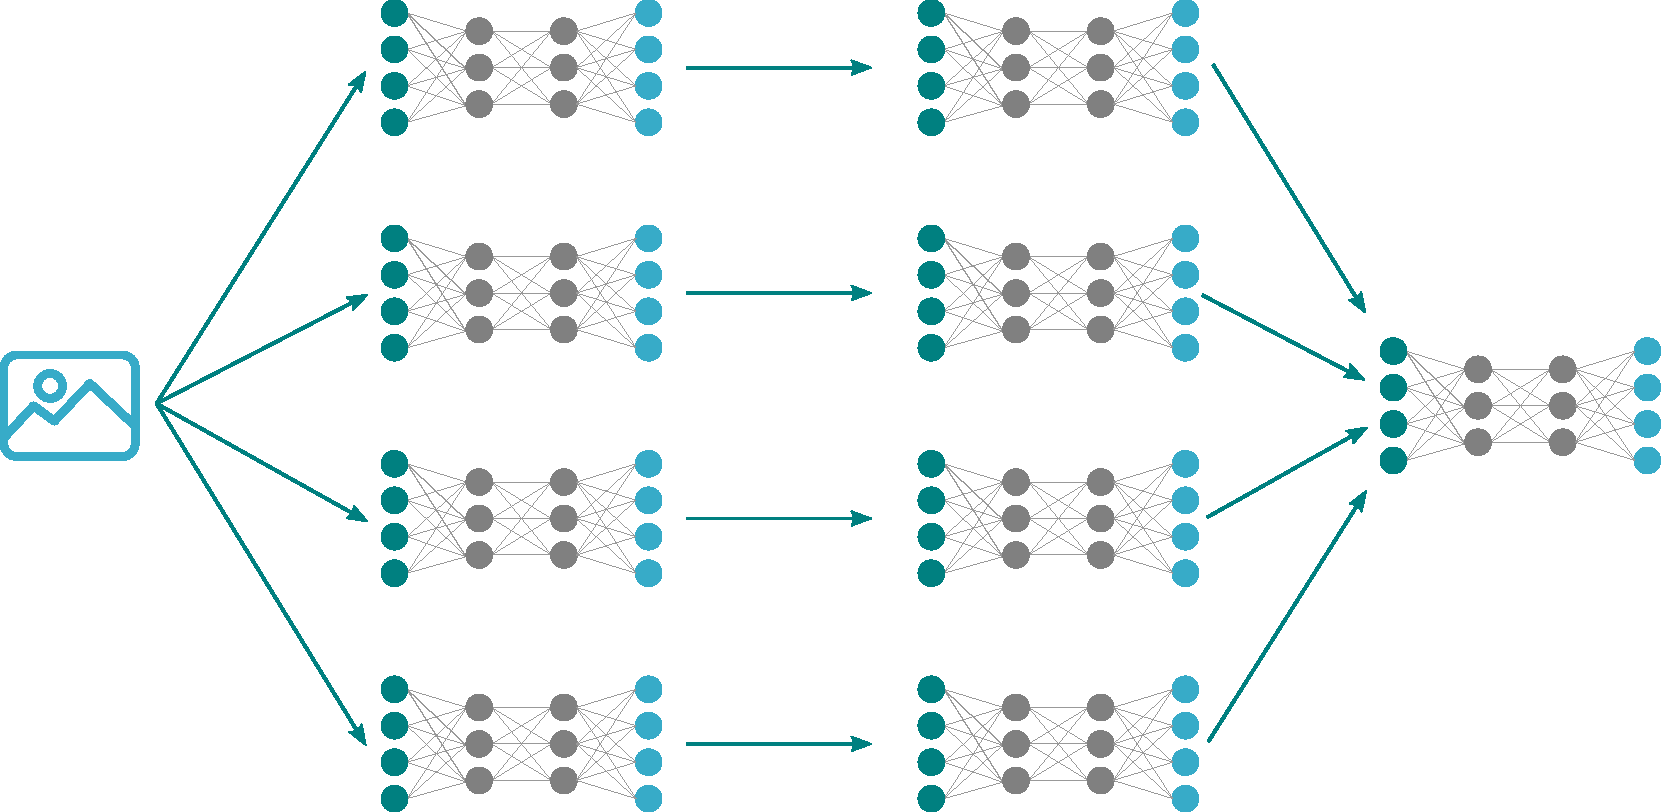
\includegraphics[width=0.7\columnwidth]{yamins_1}
	\caption{Avtor ikone slike je \cite{imageicon}. Ikono smo pridobili po licenci \url{https://creativecommons.org/licenses/by/3.0/legalcode}.}
\end{figure}

Model so zgradili iz hierarhičnega sklada enostavnih nevronskih mrež in ga optimizirali z modularno optimizacijo. Pri tej optimizaciji enostavne nevronske mreže najprej specializiramo na del celotnega problema (razpoznavanje določene kategorije). Mreže nato združimo in popravimo uteži tako, da ima celotna mreža najmanjš napako. 

Model so testirali na NRB podatkovni bazi, ki je bila originalno namenjena primerjanju nevronskih značilnosti opic in ljudi \cite{yamins2013hierarchical}. Matrike razlik so pokazale, da HMO algoritem dobro opisuje ventralni tok ljudi in opic.

Podobno so se z modeliranjem IT korteksa ukvarjali v \cite{yamins2014performance}. Tudi tu so modele zgradili iz hierarhičnega sklada enostavnih nevronskih mrež. S primerjavo med modelom in odzivom opičjih možganov so ugotovili, da se natančnost predikcije povečuje z vsakim novim slojem nevronov. Prav tako so z rezultati pokazali, da so, poleg IT korteksa, modeli podobni tudi odzivom vidnega prodročja V4 v vizualnem korteksu.

Seveda pa je sama primerjava med umetnimi nevroskimi mrežami in možganskim vidnim zaznavanjem zelo težka, saj po eni strani nimamo enotne metrike pri eksperimentiranju, po drugi  strani pa obstajajo računalniške omejitve \cite{cadieu2014the}. Zato so v \cite{cadieu2014the} uvedli nov način merjenja zmogljivosti pri razpoznavanju kategorij objektov. Natančnost razpoznavanja so določili kot funkcijo kompleksnosti razvrščevalnika in primerjali delovanje DNN-jev s primati. 

\begin{figure}[!htbp]
	\centering
	\includegraphics[width=0.7\columnwidth]{cadieu_1}
	\caption{}
\end{figure}


V svoji študiji so izoblikovali $1960$ sintetičnih slik, s katerimi so kontrolirali variacije pozicije in orientacije objektov na slikah. Ozadje je bilo določeno naključno. Eksperimente so izvajali s pomočjo dveh primatov. Vsako sliko so jima prikazali za \SI{100}{\ms} s \SI{100}{\ms} periodo brez slike. Pri tem so merili odziv v IT korteksu in opazovali pozicijo očesa živali. 

\citea{cadieu2014the} je po svoji metodi ugotovil, da imajo DNN modeli podobno, če ne celo boljšo natančnost.


Študija primerjave med nevronskimi mrežami in primati je potekala tudi v delih \cite{rajalingham2015comparison} in \cite{rajalingham2018largescale}. V prvem delu so raziskovalci večinoma primerjali opice in ljudi v drugem delu pa so se osredotočili na primerjavo med DNN-ji in primati. Tu so generirali sintetične slike na enak način kot v delu \cite{kheradpisheh2016deep}---3D modeli so bili z naključno pozicijo in orientacijo postavljeni na naravne slike. 

\begin{figure}[!htbp]
	\centering
	\includegraphics[width=0.7\columnwidth]{rajalingham_1}
	\caption{Avtor opice je \cite{monkeyicon}, avtor človeka je \cite{humanicon} avtor ikone slike je \cite{imageicon} in avtor ekrana je \cite{computericon}. Ikone smo pridobili po licenci \url{https://creativecommons.org/licenses/by/3.0/legalcode}.}
\end{figure}

Teste so v \cite{rajalingham2018largescale} izvajali  tako, da so najprej prikazali črno piko za \SI{500}{\ms}. Sledila je testna slika (\SI{100}{\ms}) z naključno pozicijo in orientacijo. Na koncu sta se prikazali še dve sliki objektov s kanoničnim pogledom izmed katerih je ena slika vsebovala testni objekt. Merjenec je nato moral izbrati eno izmed slik. Testirali so 1476 ljudi na AMT, 5 odraslih opic (Macaca mulatta) in DNN modele.

Za testiranje so uporabili naslednje vedenjske metrike:

\begin{enumerate}
	\item \emph{B.O1} Razlikovanje objekta proti vsem ostalim.
	\item \emph{B.O2} Razlikovanje objekta proti distraktorju.
	\item \emph{B.I1} Razlikovanje slike proti vsem ostalim.
	\item \emph{B.I2} Razlikovanje slike proti distraktorju.
\end{enumerate}

Rezultate so ovrednotili na podlagi normalizirane Pearsonove korelacije, kjer je izbrani vizualni sistem identičen človeškemu pri vrednosti \num{1.0}, četudi obstaja šum v podatkih. Rezultati za posamezen test so zbrani v tabeli \ref{tab:rajalingham_1}. Avtorji so odkrili, da so DNN-ji natančno določili vzorce primatov o zmedenosti med objekti (kako pogosto zmedeno razpoznamo kamelo za psa). Vendar pa, ko so raziskovali za posamezne slike, so ugotovili, da noben DNN  model ne deluje dobro. 

\begin{table}[!htbp]
	\centering
	\begin{tabular}{l S[table-format=1.3, round-mode=places, round-precision=2, table-space-text-pre=$\sim$]  S[table-format=1.3, round-mode=places, round-precision=2, table-space-text-pre=$>$]  S[table-format=1.3, round-mode=places, round-precision=2]  S[table-format=1.3, round-mode=places, round-precision=2]}
		\toprule
		\textbf{Metoda} & \thead{B.O1} & \thead{B.O2} & \thead{B.I1} & \thead{B.I2}  \\
		\midrule
		Ljudje & 0.97 & 0.94 & 0.96 & 0.77 \\
		Opice & 0.90 & 0.8 & 0.77 & 0.75 \\
		Inception-V3 & {$\sim$} 0.90 & {$>$}0.8 & 0.62 & 0.53 \\
		\bottomrule
	\end{tabular}
	\caption{}
	\label{tab:rajalingham_1}
\end{table}



